\chapter{Introduction}
\section{Optimization in Neural Networks}
Optimization is a core part of the current deep neural networks, as it is the
foundation of the learning process. However, optimization in the context of deep
learning differs from traditional optimization in several ways. This section
focuses on these differences and other current challenges of optimization in
deep neural networks. Most of the sections are inspired by
\cite{Goodfellow-et-al-2016}.

\subsection{Difference to normal optimization}\label{sub:1}
In traditional optimization, we usually optimize on the data we want to perform
later directly. However in deep learning, we usually don't have access to the
test data. Consider autonomous driving. Here, the data the self-driving agent
has to act on will be generated while driving, with no chance of getting it in
advance. But we can capture data of other cars and optimize on them indirectly.
The hope beeing, that the distribution of the training set is similar to the one
of the later test set, so that reducing training error will result in reducing
test error.

Formally, we want to reduce the test error given by
\begin{align}\label{eq:1}
    J(\theta) = E_{(x,y)\sim p_{data}} L(f(x;\theta), y)
\end{align}
where $L$ is the Loss-Function, $f(x;\theta)$ the output of the network with
respect to the input $x$ and parameters $\theta$, and $y$ the labels for the
input. This equation is known as \textbf{risk}. However, during the training
process, we only have access to the training set which is distibuted according 
to $\hat{p}_{data}$ rather than $p_{data}$. Therefore, we can only optimize
\begin{align}
    J(\theta) = E_{(x,y)\sim \hat{p}_{data}} L(f(x;\theta), y)
\end{align}
To overcome this issue, we use a technique called empirical risk minimization.

\subsection{Empirical risk minimization}\label{sub:2} As we have already seen,
although we cannot reduce the generalization risk of equation \ref{eq:1}, as we
only have the training data. To convert the problem back to a normal
optimization problem, we use the expectation over the empirical distribution.
This is known as \textbf{empirical risk minimization}. The arimethic mean
serves as an unbiased estimator for the true mean of $\hat{p}_{data}$.
\begin{align}\label{eq:3}
    J(\theta) = E_{(x,y)\sim \hat{p}_{data}} L(f(x;\theta), y) = \frac{1}{m} \sum_{i=1}^m L(f(x^{(i)}; \theta), y^{(i)})
\end{align}
As the training set from the empirical distribution is restricted in size, this
quickly leads to overfitting, where the network memorizes the training set.
Additional measurements like Regularization have to be taken to account for that
problem.

\begin{comment}
Another part in which we often optimize indirectly is the loss function
$L(f(x;\theta), y)$. Take a classification task for example. An intuitive loss
function would be the accuracy, which is computed by:
\begin{align}
    \frac{\textrm{\# of correct classifications}}{\textrm{\# of total classifications}}
\end{align}
When using this loss function with gradient descent however, this would lead to
no useful gradient as it is 0 everywhere[??]. That's why we use another loss
function like Cross-Entropy to optimize for this function indirectly.
\end{comment}

\subsection{Minibatch Algorithms}\label{sub:Minibatch}
We have seen in equation \ref{eq:3} that we use the mean over the whole training
set to approximate the empirical risk. From a computational perspective, this is
rather expensive. That's why we normally only use a subset of the training set
for each parameter update. These subsets are called batches. Some statistical
considerations justify this.

The standard error of mean is given by $\frac{\sigma}{n}$, where $n$ is the
number of training examples. The root in the denominator results in that, when
increasing the number of training examples, the standard error of mean will
only decrease sublinear. That's why it is unattractable to use large batches of
training data. The second factor is redundancy in the training set. As some
examples might be quite similar to each other, the mean of a subset will not
differ much from the whole training data, but requires much less computation
time.

Most loss-functions allow us to divide the data into batches easily. The most
common example is maximum likelyhood, which is defined as:

\begin{align}
    \theta_{ML}
    & = argmax_{\theta} p_{model}(X; \theta) \\
    & = argmax_{\theta} \prod_{i=1}^m p_{model}(x^{(i)}; \theta)
\end{align}

If we convert it to log-space, the product decomposes into a sum:

\begin{align}
    \theta_{ML} = argmax_{\theta} \sum_{i=1}^m log p_{model}(x^{(i)}; \theta)
\end{align}

In this space, we can easily divide the sum into batches and train on them
seperatly. The same idea can be applied to the gradient:
\begin{align}
    \nabla_\theta J(\theta)=E_{x,y\sim \hat{p}_{data}} \nabla_\theta log(p_{model}(x,y;\theta))
\end{align}

Optimization algorithms which use the whole trainig set are called
\textbf{batch} or \textbf{deterministic} algorithms, while deterministic is
prefered, as the term batch is also used in minibatch methods. The other extreme
are \textbf{stochastic} or \textbf{online} methods, where only one training
example is processed at a time. In between lie the methods, where more than one
training example is used, but not all. These are called \textbf{minibatch}
methods and are most commonly used in machine learning. A typical example for
stochastic methods is stochastic gradient descent (SGD), see section \ref{SGD}.


Both methods have their advantages beyond the computational perspective. While
large batches offer a more accurate estimate of the gradient, small batches can
add a regularization effect. They add some noise to the gradient, and therefore
lead the optimization algorithm to areas, where a small inaccuracy in the
gradient converges to the same point. As the point is a very stable or wide
minimum, this results in a regularization effect which decreases the
generalization error. This is also supported by the work of Keskar et al.
\cite{keskar2016large}, who argued that larger batches converge to sharp
minimas, whereas small converge to flat. As we will argue in flat minima are
believed to be better in generalization. Therefore, a small batch which ends up
in a flat minima results in better generalization capabilities.


The effect of batch size is also sensitive to the choice of the optimization
algorithm. In particular, second-order algorithms suffer from a small batch
size. Hessian matrices H require a much larger sample size to be accurate than
the Jacobian. Especially when H is of large condition number, this leads to the
an amplification of the preexisting errors in g.

To get an unbiased esimate of the gradient, it is important to sample the
mini-batches randomly. This is a problem in particular when the training data is
corellated. This may arise as autocorellation where consecutive examples are
corellated for example. The problem can be overcome by sampling the minibatches
uniformly out of the training data. However, that would lead to a large
computational effort every time we want to construct a batch. Fortunally, it
seems sufficient to shuffle and divide the training data into batches only once.

Another property is that the gradient of minibatch algorithms like SGD follow
the true gradient, as long as the training data is only used once. As each
datapoint from the training set is only used once, it also follows the true data
distribution $p_{data}$. Therefore we get an estimate of the true gradient of
the generalization error. When reusing the data from $\hat{p}_{data}$, it no
longer follows $p_{data}$, so the estimation becomes inaccurate.

\subsection{Challenges in Neural Networks}
In the last part, we demonstrated how optimization in deep learning differs from
traditional optimization from a statistical point of view. This difference is
emphasized further by other factors, in particular the non-convex loss
landscape. This part will summarize some of these problems and their
implications for deep learning.


\subsubsection{Local Minima}
In convex optimization problems, every local minima is guaranteed to be the
global minima. Therefore finding a minimum is a sufficient enough condition to
stop. In neural networks however, the loss landscape is highly non-convex. This
results in a local minima possibly having higher cost value than the global
minima. Proofs that these local minima exist can be constructed quite easily.

One example is the weight space symetrie. Suppose you swap out nodes i and j by
swapping their incoming and outgoing weights. Then the activation in the next
and all subsequent layers of the networks will stay the same, but the networks
are located at different places in the loss landscape, therefore creating two
local minimas. Although a large number of these local minima exist, they form no
problem for optimization. As mentioned, the swap will lead to the same
activation, therefore the networks will performe the same on the data and the
value of these local minimas will be equal.

However, there can also exist local minima with high cost compare to the global
minimum. In theorie this was believed to be an issue, but in practice it seemed
to cause no problem. Recently, some theoretical work support these findings.
Chromanska et al. \cite{choromanska2015loss} applied spin glass theory from
physics to neural networks. This allowed them to verify, that indeed nearly all
local minima are of roughly the same cost and lead to the same test error.
Furthermore, the propability of a local minima with high cost quickly diminishes
as the network grows in size. One reason is that most local extrema are in fact
saddle points.

\subsubsection{Saddle Points}\label{prob:3}
Saddle points are another type of local extrema where the gradient is 0. In
contrast to local maxima or minima where the Hessian only has negative or
positive eigenvalues, the Hessian of saddle points has both positive and
negative eigenvalues.

In fact, saddle points get more common for higher dimensional space. The idea of
coin flipping can be used to describe this phenomena. Suppose every eigenvalue
of the Hessian is generated by flipping a coin. In a low-dimensional space, it
quite likely that all of these flips will be positive or negative, resulting in
minima or maxima. The higher the dimension gets however, the more likely the
Hessian is to have both positive and negative eigenvalues. Therefore, there
exist more saddle points. Chromanska et al. \cite{choromanska2015loss} also
showed that these saddle points are more likely to occur in areas of higher
loss.

What problems arise from saddle points depends in the choice of the optimization
algorithm. For first-order algorithms, the situation is unclear. Although the
gradient might get small in regions close to saddle points and as a result could
slow down training, in pratice it seems like it isn't a problem for gradient
descent. Especially when adding Momentum to the algorithm, it is very unlikely
that that the gradient becomes 0, because there is no gradient in opposing
direction which would decrease the momentum.

For second-order algorithms, saddle points are clearly a problem. Newton's
algorithm for example explicitly solves for point with zero gradient, and is
therefore attracted to saddle points or even other extrema like maxima. This is
partly resolved by the introduction of saddle-free Newton. 


\subsubsection{Vanishing gradients}\label{sub:Vanishing_gradient} Today's neural
network become very deep. But with increasing depth, there arises a problem
called vanishing and exploding gradient. It refers to the fact that when
back-propagating the gradient, it either vanishes or explodes. More formally,
consider a matrix $W$ which is multiplied by repeatedly on a computation path.
If a eigendecomposition $Vdiag(\lambda )V^{-1}$ exists, this results in
$(Vdiag(\lambda )V^{-1})^t=Vdiag(\lambda )^tV^{-1}$. Therefore, all values are
scaled according to the eigenvalues of $W$. If these eigenvalues are between 0
and 1, the gradient will vanish. If they are larger then 1, it will explode.
This especially occurs when the network becomes increasingly deep, as the power
of these eigenvalues is taken. One solution for this problem is the ResNet
architecture, which will be described in detail in section \ref{sub:ResNet}

\subsubsection{Poor correspondence betwenn local and global
structure}\label{prob:5}

The previous sections have focused on which problems we are facing when
computing a gradient or updating locally. However, the local structure can often
be misleading, as it doesn't reflect the global one. Even if we are able to
perform the best move locally and end up in a local minima, we are not
guaranteed to be in the globally best area. Figure \ref{fig:Poor_correspondence}
shows an example of suboptimal initialization. As the local structure for $x<0$
doesn't reflect the global, these initializations will not lead to the global
minimum.

\begin{figure}[h]\label{fig:Poor_correspondence}
    \begin{center}
        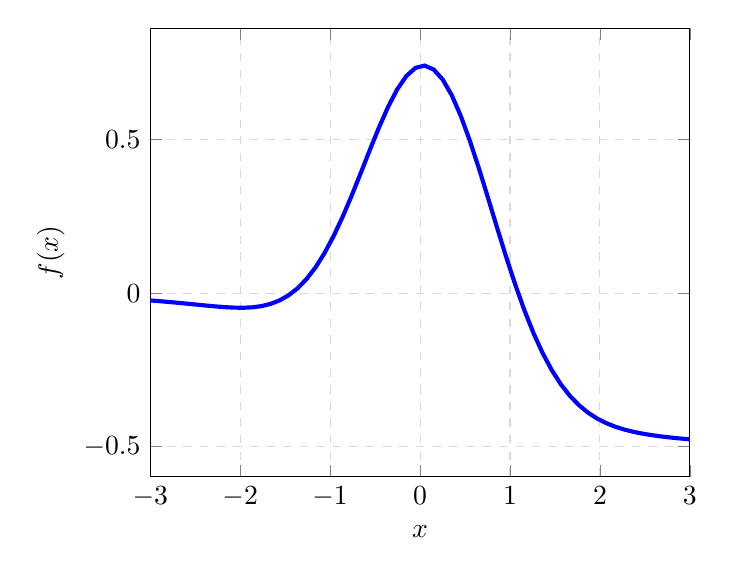
\begin{tikzpicture}
            \begin{axis}[
            grid=major, 
            grid style={dashed,gray!30},
            xlabel=$x$, % Set the labels
            ylabel=$f(x)$,
            xmin=-3,
            xmax=3]
            \addplot[mark=none,color=blue, line width=1.5pt, samples=100] {exp(-(x-0.1)^2)-0.5/(1+exp(-x))};%{exp(-x^2)-0.5*exp(-(x-2)^2)+1};
            \end{axis}
        \end{tikzpicture}
        \caption{Example of poor correspondence between local and global
        structure. If $x<0$ is initialized, gradient descent will lead us in
        negative direction. However, this leads away from the global optimum
        on the right.}
    \end{center}
\end{figure}

Another issue may be that there even is no global minimum. This happens for
example with the usage of the softmax, where the weights are increased without
bound even when the accuracy is very good. This occurs because the actual labels
for the softmax can only approach 1 with larger values, but never actually reach
it.  On solution to the second phenomena would be label smoothing, where instead
of a hard 0-1 coding of the classification, each of the 0 are replaced by
$\frac{k}{\textrm{\# of output units }-1}$, and the label for the true
classification is replaced by $1-\frac{1}{k}$. The network is now able to
resemble the labels without extreme output values.

Solutions for this problem primarly focus on choosing the right inital values at
the moment.

\subsubsection{Initialization strategies}\label{sub:Initialization_strategies}
In the last section, the poor correspondence between local and global structure
was shown. Initializations at the wrong place on the loss landscape lead to a
gradeint descent in a direction away from the global optimum. But as we don't
know the shape of the loss landscape in advance, no initialization can guarantee
a good solution or even convergence at all. Hwowever, some strategies have
become widely used.

The first and only known property of initialization is that is has to be
asymetric. This means that two units that share the same input must have
different weights attached to these inputs. If this is not the case, a
deterministic optimization algorithm, will update both these parameters in the
same way. To break this symetry, the weights are initialized randomly. If a
gaussian or uniform distribution is used doesn't really seem to matter.

However, the range of these functions seems to matter. Wide distributions have a
stronger symetry breaking effect, but come with the risk of exploding gradients
as discussed in section \ref{sub:Vanishing_gradient}. The problem of vanishing
gradients arise if the distribution is too small. The statictical viewpoint
suggests a initialization to small weights nevertheless. Here, large weight
initialization is seen as a large gaussain prior, which and how the units
interact. As we have no reason to encourage one interactionover another, the
weights should be as small as possible. 

Some heuristics try to balance these different motivations. One of the most
famous one is the normalized initialization from Glorot
\cite{glorot2010understanding}. For a fully connected layer of $m$ inputs and
$n$ outputs, the weights should be initilaized according to a uniform
distribution:

\begin{align}
    W \sim U(-\sqrt{\frac{6}{m+n}}, \sqrt{\frac{6}{m+n}})
\end{align}

The biases are normally initialized to a constant. A value of 0 seems to behave
well for most applications.




\subsubsection{Stopping criteria}
In traditional optimization, simple heuristics are used to determine the point
of stopping, like a gradient of 0. However many local minima exits on the loss
landscape. In addition, usually we are notable to find these local extrema, as
minibatch algoprithms only give an approximation of the real gradient and the
learning rate may lead to large step sizes which overshoot the minimum.

What we normally see in terms of performance is an initial decrease in training
loss paired with an increase in validation accuracy. But after some epochs, we
enter the overfitting region, where training loss keeps decreasing but
validation accuracy also decreases again. In early stopping, this is used the
determine the stopping point. After each epochs we store a copy of the parameter
values. Then we train the network for a fixed number of epochs. At the point when
the validation error starts to rise again, we can return to the parameters
before. As no additional computation time is required, this is a very efficient
method from a computational perspective, but may require some extra storage.
This apporach is very different to traditional optimization,as gradients may
still be very large.



\subsection{Algorithms}
\subsubsection{Stochastic Gradient Descent}\label{SGD}
Stochastic Gradient Descent is one of the most popular optimization algorithm in
deep learning. It is also one of the most basic ones, as it only takes the
gradient at the current position into account. In contrast to normal gradient
descent, SGD computes the gradient on minibatches, not on the whole dataset.
Nevertheless, as long as the training data is only used once, SGD gives an
unbiases estimate of the true gradient (see Section \ref{sub:Minibatch}). 

\begin{algorithm}\label{alg:SGD}
    \begin{algorithmic}[1]
        \caption{Stochastic gradient descent from \cite{Goodfellow-et-al-2016}}
        \REQUIRE learning rate $\epsilon$
        \ENSURE a trained neural network
        \STATE initialize the network, dataset and training parameters
        \WHILE{stopping criteria is not met}
            \STATE sample minibatch of $m$ examples ${x^{(1)}, ... ,x^{(n)}}$
            \STATE compute gradient estimate $\hat{g}=\frac{1}{m} \nabla_\theta \sum_i L(f(x^{(i);\theta}),y^{(i)})$
            \STATE apply parameter update $\theta=\theta-\epsilon\cdot\hat{g}$
        \ENDWHILE
        \STATE \textbf{return: the trained network}
    \end{algorithmic}
\end{algorithm}

First, the network is initialized. Then, the training loop repeats, until the
stopping criteria is met. At the beginning, a minibatch is sampled. Then, the
gradients are calculated, multiplied by the learning rate $\epsilon$ and finally
applied to update the parameter values.


\subsubsection{Learning rate decay}\label{sub:Learing_rate_decay}
One of the most important hyperparameters of SGD is the learning rate. While the
optimal learning rate differs for every problem, it is important to decay the
learning rate with the number of epochs. Initilally, it is good to choose a
large learning rate. This leads to fast learning at the beginning, and avoids
the algorithm getting stuck areas of high loss. As the number of epochs
increases, it is important to shrink the learning rate. SGD only is a stochastic
algorithm, therefore its gradient is inaccurate. Even when we find a local
minima with a gradient of 0 on the minibatch, the true gradient will not be 0. A
low learning rate secures to get close to the minimum while not overshooting it
repeatedly.

[TODO: Formula 8.12, 8.13] How the learning rate is decayed varies from
algorithm. A popular decay is step decay, where the learning rate is decayed by
a constant factor $\gamma$ after a fixed number of epochs.
\begin{align}
    lr = lr_0 \cdot \gamma^{\lfloor epoch/stepsize \rfloor}
\end{align}
Another popular algorithm is cosine decay, where the learning rate is decayed
continously.
\begin{align}\label{eq:cosine_decay}
    \epsilon_t = \epsilon_{min} + \frac{1}{2} (\epsilon_{max} - \epsilon_{min})(1+cos(\frac{T_{cur}}{T_0}\pi))
\end{align}
Here $\epsilon_{min}$ and $\epsilon_{max}$ define the range of the lr, $T_cur$
is the current and $T_0$ is the maximum number of epochs. The advantage of
cosine decay is that the learning rate is decayed down to 0 in the defined
interval, independent of the initial learning rate. In contrast, the smallest
learning rate of step decay is dependent of the initial  one.

\subsubsection{Momentum}\label{sub:Momentum}
Momentum is a popular variation of SGD. It is used to speed up the training of
SGD. The term momentum is used, as the underlying idea is the similar to the
physical context. Consider a frictionless ball rolling down a hill. The ball
builds up speed the further it rolls down by adding the acceleration of current
gradient to the velocity. The ball will speed up, until it faces an uphill,
where it will slow down again.

In context of deep learning, we use the velocity $v$ rather than only the
current gradient $g$ to update the parameters.

\begin{align}
    v_{t+1}=\alpha v_t - \epsilon g
\end{align}
Here, $\alpha$ controls how strong the past gradient is taken into account,
while $\epsilon$ denotes the current learning rate. For the ball to build up
velocity, it requires a constant downhill motion. The same is true for this
case. The gradient can only build up, if it points in the same direction for
some consecutive updates similar to a ball, which only speeds up when rolling
downhill for an amount of time. Therefore, momentum speed up the gradients of
parameters, whose gradient is constant in one direction. Parameters with
alternating gradients for example will only experience small updates. The
different orientations of their gradient will level out. Formally, if parameter
p experiences the same gradient g every time, it will reach a terminal velocity
of
\begin{align}
    \frac{\epsilon \lVert g \rVert}{1-\alpha}
\end{align}
This also shows that $\alpha$ can be used to control the speed up of the
training. If $\epsilon$ is kept constant, the larger $\alpha$, the faster
training will become. An value of $0.9$ for example would lead to a speed up
factor of $10$, while $0.8$ would lead to a speed up of $5$.

\begin{algorithm}
    \begin{algorithmic}[1]
        \caption{Stochastic gradient descent with Momentum from \cite{Goodfellow-et-al-2016}}
        \REQUIRE learning rate $\epsilon$
        \REQUIRE momentum parameter $\alpha$
        \ENSURE a trained neural network
        \STATE initialize the network, dataset and training parameters
        \WHILE{stopping criteria is not met}
            \STATE sample minibatch of $m$ examples ${x^{(1)}, ... ,x^{(n)}}$
            \STATE compute gradient estimate $\hat{g}=\frac{1}{m} \nabla_\theta \sum_i L(f(x^{(i);\theta}),y^{(i)})$
            \STATE compute velocity update $v=\alpha v - \epsilon \hat{g}$
            \STATE apply parameter update $\theta=\theta-v$
        \ENDWHILE
        \STATE \textbf{return: the trained network}
    \end{algorithmic}
\end{algorithm}

In pseudo code, SGD with Momentum looks similar to normal SGD \ref{alg:SGD}. The
only difference is line 5 and 6, where the velocity is updated and then used to
update the parameters rather than the gradient itself.


Momentum also adds an regularization effect, because it is attracted to stable
or flat minima. If the minima is too small, it won't be able to stop the
momentum and therefore the SGD will move on. That's similar to a ball, which
won't stay in a small hole but keep on going, if it's speed is larger enough.






\section{Related work}
\subsection{Generalization gap}\label{sub:Generalization}
In section \ref{sub:1}, we saw how learning differs from normal optimization,
namely that we only have acces to the training set and thus have to optimize
indirectly. With an increasing number of training epochs, the network starts to
memorize the training data. Because the data distribution of the training data
is not identical to the distribution of test data, this usually leads to a
better performance of the network on the training set than on the test set. The
difference between those performances is known as Generalization gap. 

Strategies that are developed to deal with this problem are subsumed under the
term \textbf{regularization}. One common Reguralizer is the $L_2$ Reguralizer.
It's goal is, to encourage the weights to stay small. Small weights have some
advantages for the generalization capabilities. First of all, small weights
remove the dependency of a unit to one of it's inputs. Because the weights are
really small, a strong activation cannot be solely achieved by the presence of
one input, but rather has to rely on multiple units. Therefore small changes in
the input will only cause small changes in the output, instead of the absence of
one feature for example leading to a different output. This benefits the
generalization, as the distribution of training and test data is slightly
different. A network with $L_2$ regularization will nevertheless produce a quite
similar output, in contrast to a normal one. Formally this can be incorporated
in the loss function by adding the squared $L_2$ norm:
\begin{align}
    L= L(f(x;\theta), y)+\lambda \cdot \lVert \theta \rVert_2^2
\end{align}
The paramter $\lambda$ controls the strength of the $L_2$ and has to be adjusted
for each problem.

Other work has gone into understanding the connection to the loss surface.
Hochreiter \& Schmidhuber \cite{hochreiter1997flat} argued that flat minimas
have better generalization capabilities. A flat minima is a region where the
loss stays constant in conrtrast to sharp one, where small steps can increase
the loss significantly. Therefore, flat minimas will perform constantly even for
small changes in the input, whereas sharp minimas will lead to an increase in
generalization error. Support also comes from the minimum description length
theory, which states that fewer bits are needed to describe a flat minimum than
a sharp. Lower complexity leads to a better generalization error. The idea is,
that in the network we try to compress the data. The more we compress the data
while also beeing able to resemble it, the more of the structure of the data we
uncover. Therefore, a model with lower complexity can fit the underlying data
better and achieve a better generalization error. Keskar et al.
\cite{keskar2016large} draw the same conclusion. They also provide a solution
for finding flat minimas in using small batch sizes, see chapter
\ref{sub:Minibatch}.

Work from Dinh et al. \cite{dinh2017sharp} however contradicts this view. They
argue that the notion of flat is problematic in the context of deep learning, as
the loss surface is highly complex. Based on previous definitions from the
papers above, they construct parameter values which lie on a sharp point of the
surface, but are also able to generalize well. Therefore, at least some caution
in needed when arguing about flatness beeing a reason for generalization
capabilities.

\subsection{Areas of same loss}\label{loss_landscape}
In section \ref{prob:5}, we showed that the poor correspondence between local
and global structure may propose a major issue for optimization. Bad
initializations may lead to path which moves away from the global otimum, often
without chance to recover. Initialization strategies try to adress this problem,
but cannot guarantee to solve it.

An open question is if this suboptimal structure is present in deep neural
networks. Fengxiang et al. \cite{he2020piecewise} showed that there exists
infinetly many local minima which are of higher cost than the global one.
Furthermore, these minima are arranged in cells, where each minima of one cell
is of same loss as the others and also connected with them by valleys of low
loss. These cells are seperated by nondifferentiable boundaries. Unfortunally,
it remains unclear if these cells are of different cost. If this is the case,
this would propose a major problem. When the training process gets into one of
these cells, it is likely to get stuck, probably in an area of suboptimal cost.
A trivial way to recover is not present at the moment.

Draxler et al. \cite{draxler2018essentially} get to a smiliar result, that local
minimas are connected by valleys. In these valleys, the training loss stays the
same to the one of the connected minima, while the test error rate slighly
increases.

Fort \& Jastrzebski \cite{fort2019large}  this in a more formal context. For
each tuple of dimensions, they construct disks to describe the hyperplanes
defined by them. They calls these hyperplanes wedges. One property is that the
valleys of low loss described above lay on these wedges. Therefore the
connecting valley for two points on different wedges has to pass through the
intersection of them. When viewed from an cross-section, these valleys from a
tunnel. Some techniques to improve optimization have similar effects on the size
of these tunnels, namely they widen them. This happens for example for higher
$L_2$ regularization \ref{sub:Generalization}, smaller batch sizes
\ref{sub:Minibatch} or higher learning rates.


\subsection{Cosine decay with warm restart}\label{sub:cosine_decay}

In section \ref{SGD}, we introduced learning rate schedulers. The idea was to
have a high learning rate at the beginning for fast improvements, and then an
decrease to fine adjust the parameters. On scheduler was cosine decay, with the
formula \ref{eq:cosine_decay}. In the paper of Loshchilov \& Hutter
\cite{loshchilov2016sgdr}, they use this scheduler in combination with another
technique, called warm restart. In constrast to the naive approach, where the
learning rate is only decayed once, warm restart decayes until a fixed number of
epochs, and then set back up to the inital learning rate. This procedure can be
repeated for several times. The idea is, that in phases of high learning rate,
the network explores the loss surface due to large steps. In epochs of low
learning rate, the network exploits a small area to find the best parameter
values. This may also add an regularization effect by letting the optimizer
escape from unstable minima during high learning rate. [doubtful???]

The authors report an new state of the art result at 3.14\% test error for
Wide-Residual-Net 28-20. Their method also perfoms better when compared to step
decay.
\subsection{Ensemble methods}\label{sub:Ensemble_Methods}
The general idea of ensemble methods is to combine the predictions of multiple
networks to get a more accurate prediction. The fact that this leads to an
improvement can be seen in a simple regression problem. Suppose there exist k
models that make an error of $e_i$ with mean 0, variance $E[e_i^2]=v$ and
covariances $E[e_i e_j]=c$ on every particular prediction. If these models are
combined, the variance reduces to 
\begin{align}
    E[(\frac{1}{k} \sum_i e_i)^2]=\frac{1}{k^2}E[\sum_i (e_i^2 + \sum_{j\neq i} e_i e_j)]=\frac{1}{k}v+\frac{k-1}{k}c
\end{align}
If all models make the same predictions, so $c=v$ for all combinations of
models, then the sum decomposes to $v$, so the prediction error is the same as
before. On the other hand, if $c=0$, the prediction error is reduced by a factor
of $\frac{1}{k}$. Therefore, for ensemble methods to be succesfull, every model
has to achieve a low prediction error, while the predictions of all models
should be as different as possible. While the low error is achieved in deep
learning by standard training of the models, there are several approaches to
ensure that these models are different. 

The first idea would be to vary the training data for the model. One way this
can be realized is by k-fold cross-validation. Here, we split the training data
into k different smaller datasets. Then we train k independent networks on one
of these subsets. This however decreases the size of the training set for each
model drastically. Therefore another common approach is bagging
\cite{breiman1996bagging}, where we draw a subset from the training data, but
with replacement. Here, individual examples might occur in more than one
training set. Training on different datasets leads to different models, which we
can use to our advantage as we have seen above. As the number of training
examples is limited however, we might not be able to sustain a sufficient low
error.

To use the whole training data while also creating different models, we can
alternatively alter the model itself. An naive approach would be to just use
different model architectures. If we want to use the same architecture for all
models, we can vary the parameter initilializations. This is often enough to
create models that have different predictions. However, for every initialization
a network has to be trained from beginning, which can become very costly. A
novel approach is to train one network, but to take snapshots of the network
parameters at different steps. This approach adds no additional cost, as we only
train one network. To ensure different networks, Huang et al.
\cite{huang2017snapshot} use the method of cosine decay with warm restarts
\cite{loshchilov2016sgdr}, as explained in section \ref{sub:cosine_decay}.
Recall that at each restart, the learning rate is set up to the initial learning
rate. This results in the optimizer taking larger update steps and consequently,
the network parameter values will distance from their current state. The
snapshots of the networks are taken before each restart, as the network
converges to area of low loss when the learning rate is low. With this method,
we are able to get different models with low error and no additional cost.

After we have ensured that the conditions for the models are met, we have to
think about how to combine these predictions. For the case of classification
with the use of softmax layer, we can use a technique called model averaging.
Here, we sum the predictions of the individual models, and take the class with
the highest prediction, as in standard classification. Formally, if the
probability output of a model i for a given class c is $p_{c_i}$, then we sum
the propabilites of each individual model: $p_c = \sum_i p_{c_i}$. To predict
the class we take $argmax_c(p_c)$. If we have reasons to believe in a better
prediction of one model over another, we can add weights $w_i$ to the
propabilites of the individual models: $p_c = \sum_i w_i \cdot p_{c_i}$.


\begin{comment}
Further aspects that could be included:
- classififcation in general
- cross entropy loss and loss functions
- gradient descent


openquestions:
where generalization gap
areas ofsame loss better
expand sgd warm restart


\end{comment}